\documentclass[12pt,a4paper]{article}
\usepackage[utf8]{inputenc}
\usepackage[english,russian]{babel}
\usepackage{amssymb,amsfonts,amsmath,cite,enumerate,float,indentfirst}
\usepackage{graphicx}
\usepackage{geometry}
\usepackage{systeme}
\usepackage{hyperref}
\usepackage{url}
\hypersetup{
	colorlinks,
	citecolor=black,
	filecolor=black,
	linkcolor=black,
	urlcolor=black
}
\geometry{left=2cm}
\geometry{right=1.5cm}
\geometry{top=2cm}
\geometry{bottom=2cm}

\begin{document}
	
\begin{titlepage}
	\begin{center}		
		\vfill	
		Санкт-Петербургский политехнический университет \\
		Петра Великого\\
		\vskip 1cm
		Институт прикладной математики и механики \\
		Кафедра «Прикладная математика»
		\vfill
		\textbf{Отчёт\\
			по лабораторной работе №1\\
			по дисциплине\\
			«Математическая статистика»\\}
		\vfill
	\end{center}
	\vfill
	\hfill
	\begin{minipage}{0.4\textwidth}
		Выполнил студент:\\
		Самутичев Евгений Романович\\
		группа: 3630102/70201\\
	\end{minipage}
	\vfill
	\hfill 
	\begin{minipage}{0.4\textwidth}
		Проверил:\\
		к.ф.-м.н., доцент\\
		Баженов Александр Николаевич\
	\end{minipage}
	\vfill
	\begin{center}
		Санкт-Петербург\\2020 г.
	\end{center}
\end{titlepage}

\tableofcontents
\listoffigures
\pagebreak

\section{Постановка задачи}
Для каждого из 5 распределений:

\begin{enumerate}
	\item Нормального $N(x, 0, 1)$
	\item Коши $C(x, 0, 1)$
	\item Лапласа $L(x, 0, \frac{1}{\sqrt{2}})$
	\item Пуассона $P(k, 10)$
	\item Равномерного $U(x, -\sqrt{3}, \sqrt{3})$	
\end{enumerate}

сгенерировать массив случайных данных (выборку) размера: 10, 50, 1000 и построить графики плотности вероятности (функции вероятности для распределения Пуассона как дискретного).

\pagebreak

\section{Теория}
\subsection{Распределения}
Пусть задано вероятностное пространство $(\Omega, \mathcal{F}, \mathbf{P})$, на котором определена \textit{случайная величина} $\xi:\Omega\to\mathbb{R}$ т.е. функция $\xi(\omega)$ такая что $\xi^{-1}(B)\in\mathcal{F},\forall{B\in\mathcal{B}(\mathbb{R})}$. Она индуцирует вероятностную меру на $\mathbb{R}$ как $\mathbf{P}_\xi(B)=\mathbf{P}(\xi^{-1}(B))$ которая и носит название \textit{распределения вероятностей} случайной величины\cite{shiryaev}.

Функция $F_\xi(x)=\mathbf{P}_\xi\mathopen{(-\infty}, x\mathclose{ ] },x\in\mathbb{R}$ называется \textit{функцией распределения} случайной величины $\xi$. Случайная величина может быть:

\begin{enumerate}
	\item \textit{дискретной}, если распределение представимо в виде $\mathbf{P}_\xi(B)=\sum\limits_{k:x_k\in{B}}{p(x_k)}$, где \newline
	$p(x_k)=\mathbf{P}_\xi{\{ x_k \}}$ для конечного $\{x_1, ..., x_n\}$ или счетного 
	$\{x_1, ..., x_k, ...\}$ подмножества вещественных чисел. В этом случае функция $p(x_k)$ называется таблицей распределения.
	
	\item \textit{непрерывной}, если $F(x)$ непрерывна
	
	\item \textit{абсолютно непрерывной}, если существует такая неотрицательная функция $f_\xi(x)$ называемая \textit{плотностью вероятности}, что $F(x)=\int\limits_{-\infty}^{x}{f(y)dy}$
\end{enumerate}

В работе рассматриваются следующие распределения:

\begin{enumerate}
	\item \textit{Нормальное} $N(x, 0, 1)$ - абсолютно непрерывное, задается плотностью
	\begin{equation}
	f_N(x)=\frac{1}{\sqrt{2\pi}}e^{-\frac{x^2}{2}}
	\end{equation}
	
	\item \textit{Коши} $C(x, 0, 1)$ - абсолютно непрерывное, задается плотностью
	\begin{equation}
	f_C(x)=\frac{1}{\pi(x^2+1)}
	\end{equation}
	
	\item \textit{Лапласа} $L(x, 0, \frac{1}{\sqrt{2}})$ - абсолютно непрерывное, задается плотностью
	\begin{equation}
	f_L(x)=\frac{1}{2\sqrt{2}}e^{-\frac{1}{\sqrt{2}}|x|}
	\end{equation}
	
	\item \textit{Пуассона} $P(k, 10)$ - дискретное, задается на $\{1, 2, ..., k, ...\}$ как
	\begin{equation}
	p(k)=\frac{10^k}{k!}e^{-10}
	\end{equation} 
	
	\item \textit{Равномерное} $U(x, -\sqrt{3}, \sqrt{3})$ - абсолютно непрерывное, задается плотностью 
	\begin{equation}
	f_U(x) = 
	\begin{cases}
	\frac{1}{2\sqrt{3}} &\text{если $x \in \mathopen[-\sqrt{3}, \sqrt{3}\mathclose] $}\\
	0 &\text{иначе}
	\end{cases}
	\end{equation}	
\end{enumerate}

\subsection{Гистограмма}
Все приведенные распределения характеризуются таблицей (для дискретных) или плотностью (для абсолютно непрерывных). Эмпирическим аналогом таблицы или плотности является \textit{гистограмма}\cite{chernova}. Гистрограмма строится по группированным данным. Предполагаемую область значений случайной величины $\xi$ делят на некоторое количество интервалов:

Пусть $A_1, ..., A_k$ - интервалы на прямой. Обозначим $\nu_j,j\in\{1, ..., k\}$ - число элементов выборки, попавших в интервал $A_j$. Размер выборки в этих обозначениях равен $n=\sum\limits_{j=1}^{k}{\nu_j}$. На каждом из интервалов строят прямоугольник, площадь которого пропорциональна $\nu_j$, общая площадь всех прямоугольников должна равняться единице (нормировка гистограммы), поэтому высота каждого определяется как $f_j=\frac{\nu_j}{nl_j}$. Полученная фигура из объединения прямоугольников и называется гистограммой.
\pagebreak

\section{Реализация}
Работа выполнена с использованием языка \textbf{Python} в интегрированной среде разработки \textbf{PyCharm}, были задействованы библиотеки:

\begin{itemize}
	\item \textbf{NumPy} - работа с массивами данных
	\item \textbf{SciPy} - модуль \textbf{stats} для генерации данных по распределениям
	\item \textbf{Matplotlib} - отрисовка гистограмм и графиков плотности/функции вероятности
\end{itemize}

Для случайной генерации было выбрано зерно 102 (для повторяемости в дальнейших экспериментах), исходный код работы приведен в приложении. Число интервалов гистограммы выбрано как округление к большему к целому $\sqrt{n}$, где $n$ - размер выборки.
\pagebreak

\section{Результаты}
\subsection{Гистограммы и графики}
\begin{figure}[h!]
	\centering
	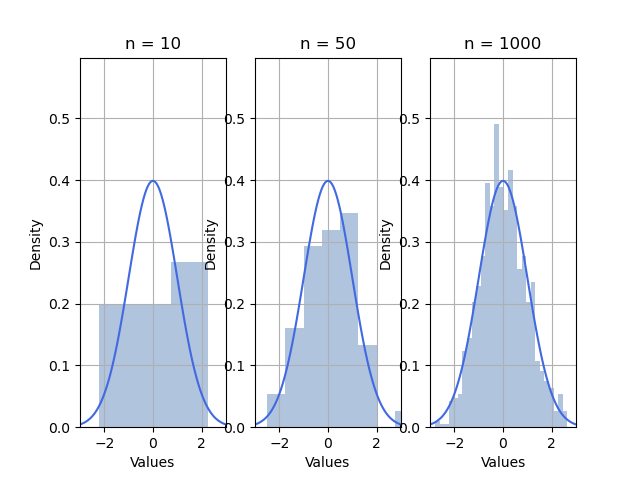
\includegraphics[scale=0.8]{normal.png}
	\caption{Нормальное распределение}
	\label{fig:image}
\end{figure}

\begin{figure}[h!]
	\centering
	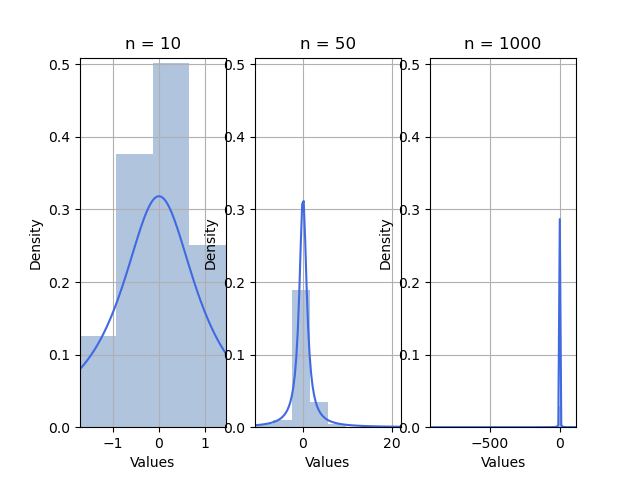
\includegraphics[scale=0.8]{cauchy.png}
	\caption{Распределение Коши}
	\label{fig:image}
\end{figure}

\pagebreak

\begin{figure}[h!]
	\centering
	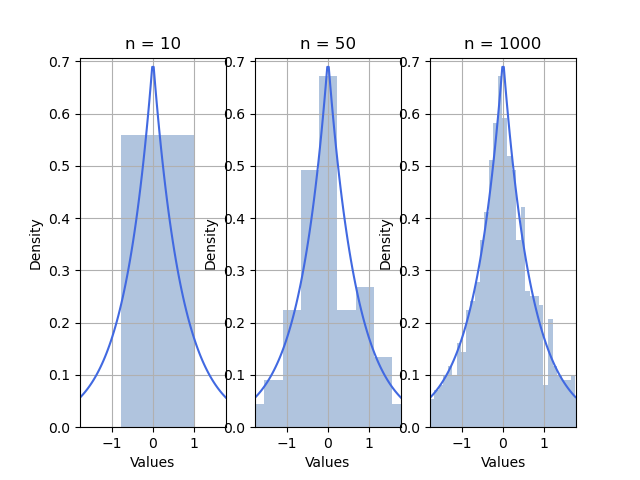
\includegraphics[scale=0.8]{laplace.png}
	\caption{Распределение Лапласа}
	\label{fig:image}
\end{figure}

\begin{figure}[h!]
	\centering
	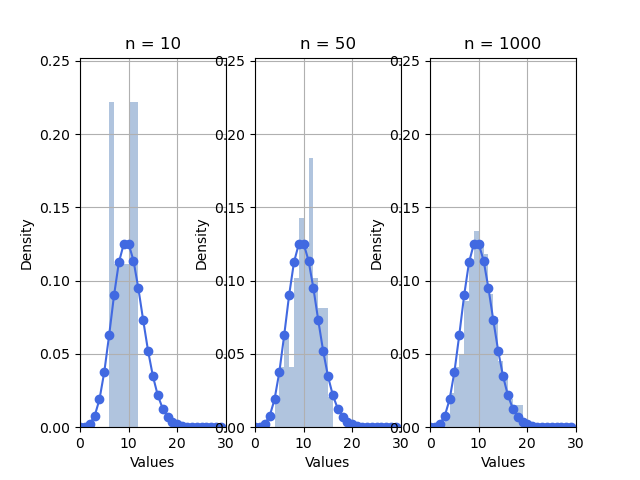
\includegraphics[scale=0.8]{poisson.png}
	\caption{Распределение Пуассона}
	\label{fig:image}
\end{figure}

\pagebreak

\begin{figure}[h!]
	\centering
	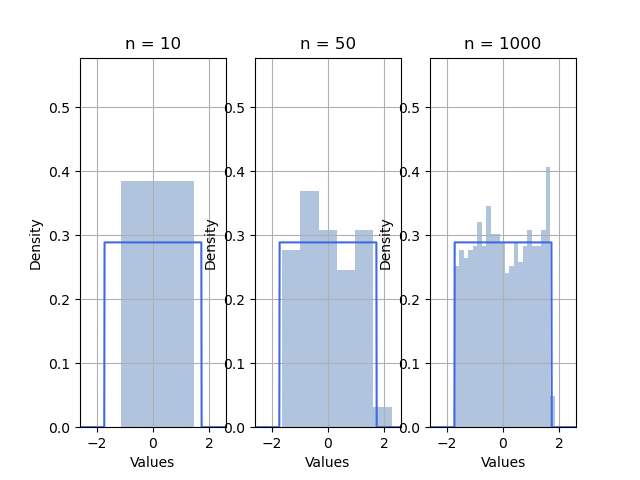
\includegraphics[scale=0.8]{uniform.png}
	\caption{Равномерное распределение}
	\label{fig:image}
\end{figure}
\pagebreak

\section{Обсуждение}
Проведенный эксперимент подтверждает \textbf{утверждение}: \textit{пусть плотность распределения по которому построена выборка является непрерывной функцией. Если число интервалов гистограммы $k(n)$ стремится к бесконечности таким образом что $\lim\limits_{n\to\infty}{\frac{k(n)}{n}}=0$, то имеет место сходимость по вероятности гистограммы к плотности.}\cite{chernova} Действительно мы взяли $k(n)=\lceil\sqrt{n}\rceil$ и очевидно условие утверждения в таком случае выполнено, при этом гистограмма при увеличении $n$ заполняет площадь под графиком плотности (кусочно-линейной функции вероятности для распределения Пуассона), а это и означает сходимость по вероятности.
\pagebreak

\section{Приложения}
\noindent 1. Исходный код лабораторной {\url{https://github.com/zhenyatos/statlabs/tree/master/Lab1}}

\begin{thebibliography}{9} 
	\addcontentsline{toc}{section}{Список литературы}
	\bibitem{shiryaev} А. Н. Ширяев, \emph{Вероятность-1}. Изд. МЦНМО, Москва, 2017. 551 стр. 
	
	\bibitem{chernova} Н. И. Чернова, \emph{Математическая статистика: Учеб. пособие}. Новосиб. гос. ун-т. Новосибирск, 2007. 148 стр.
\end{thebibliography}

\end{document}
